%!TEX root = ../graduate-work.tex

\section{Определение и свойства интеграла Римана}

\subsection{Классическое определение}

Пусть дана функция \( f(x) \), определённая на отрезке \( [a, b] \), где \(a <
b\). Разбиение отрезка \( [a, b] \) на \( n \) частей будет состоять из
последовательности точек \( a = x_0 < x_1 < \dots < x_n = b \), которая делит
интервал \( [a, b] \) на подынтервалы \( [x_{i-1}, x_i] \), где \( i = 1, 2,
\dots, n \). Каждый подынтервал имеет длину \( \Delta x_i = x_i - x_{i-1} \).

Для каждого подынтервала выбирается произвольная точка \( x_i^* \), в которой
функция \( f(x) \) оценивается. Сумма Римана для функции \( f(x) \) относительно
разбиения \( P = \{ x_0, x_1, \dots, x_n \} \) и точек \( x_i^* \) на каждом
подынтервале записывается как:

\[ S(f, P) = \sum_{i=1}^{n} f(x_i^*) \Delta x_i.  \]

Интеграл Римана функции \( f(x) \) на отрезке \( [a, b] \) определяется как
предел этой суммы, когда максимальная длина интервала \( \|P\| \) стремится к
нулю, то есть:

\[ \int_a^b f(x) \, dx = \lim_{\|P\| \to 0} S(f, P), \]

где \( \|P\| \) — максимальная длина подынтервала в разбиении \( P \).

Если этот предел существует, то функция \( f(x) \) называется интегрируемой в
смысле Римана на отрезке \( [a, b] \), и её интеграл на данном интервале
существует.

\begin{figure}[h]
\center{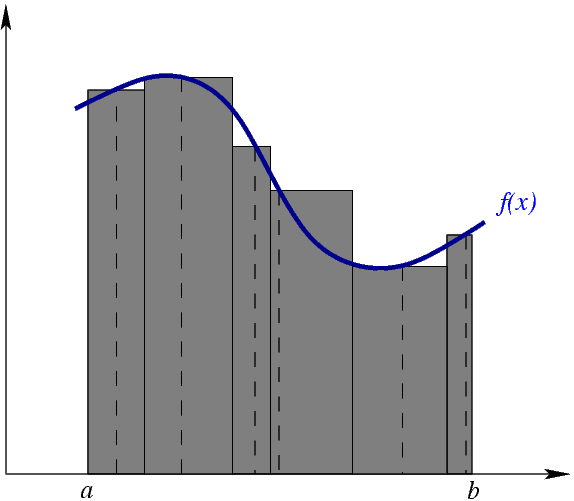
\includegraphics[width=1\linewidth]{integral}}
\caption{Геометрический смысл интеграла Римана }
\end{figure}

\subsection{Общие соображения об условиях интегрируемости}

Для того чтобы функция \( f(x) \) была интегрируемой в смысле Римана на отрезке
\( [a, b] \), она должна удовлетворять некоторым условиям. Во-первых, функция \(
f(x) \) должна быть ограниченной на отрезке \( [a, b] \). Во-вторых, она не
должна иметь слишком много разрывов. Точное требование состоит в том, что \(
f(x) \) должна быть ограниченной и иметь конечное число разрывов на
рассматриваемом интервале.

Пример функции, не интегрируемой по Риману, — это функция Дирихле на интервале
\( [0, 1] \), которая принимает значение 1 для рациональных чисел \( x \) и 0
для иррациональных чисел. Эта функция имеет бесконечно много разрывов, и её
интеграл по Риману не существует.

\subsection{Свойства интеграла Римана}

Интеграл Римана обладает рядом важных свойств, которые делают его удобным
инструментом для анализа функций. Рассмотрим несколько из них.

\subsubsection{Линейность}

Интеграл Римана обладает свойством линейности. Если \( f(x) \) и \( g(x) \) —
интегрируемые функции на отрезке \( [a, b] \), то линейная комбинация этих
функций также будет интегрируемой, причём интеграл линейной комбинации равен
линейной комбинации интегралов:

\[ \int_a^b \left( c_1 f(x) + c_2 g(x) \right) \, dx = c_1 \int_a^b f(x) \, dx +
c_2 \int_a^b g(x) \, dx, \]

где \( c_1 \) и \( c_2 \) — произвольные константы.

\subsubsection{Аддитивность}

Интеграл Римана обладает свойством аддитивности. Если отрезок \( [a, b] \)
разбить на два подынтервала \( [a, c] \) и \( [c, b] \), то интеграл на всём
интервале \( [a, b] \) равен сумме интегралов на этих подынтервалах:

\[ \int_a^b f(x) \, dx = \int_a^c f(x) \, dx + \int_c^b f(x) \, dx.  \]

Это свойство позволяет вычислять интеграл функции на сложном интервале, разбив
его на более простые части.

\subsubsection{Монотонность}

Если функция \( f(x) \) меньше или равна функции \( g(x) \) на всём интервале \(
[a, b] \), то интеграл функции \( f(x) \) меньше или равен интегралу функции \(
g(x) \):

\[ \int_a^b f(x) \, dx \leq \int_a^b g(x) \, dx.  \]

Это свойство является полезным при сравнении интегралов различных функций.

\subsubsection{Интегрируемость композиции}

Если функция \( f(x) \) интегрируема на отрезке \( [a, b] \), а функция \( g(x)
\) непрерывна на этом отрезке, то композиция \( f(g(x)) \) также будет
интегрируемой на \( [a, b] \).

\subsubsection{Интеграл и предел}

Если функция \( f(x) \) интегрируема на \( [a, b] \), а последовательность
функций \( \{ f_n(x) \} \) сходится к функции \( f(x) \) почти всюду на
интервале \( [a, b] \), то при условии, что последовательность \( \{ f_n(x) \}
\) ограничена, верно:

\[ \lim_{n \to \infty} \int_a^b f_n(x) \, dx = \int_a^b \lim_{n \to \infty}
f_n(x) \, dx = \int_a^b f(x) \, dx.  \]

Это свойство известно как теорема о пределе интегралов и является важным
инструментом для анализа предельных процессов.
